\documentclass{beamer}
\usetheme{CambridgeUS}

\usepackage{graphicx}
\usepackage{subcaption}
\usepackage{natbib}
\usepackage{booktabs}

\DeclareMathOperator*{\argmin}{argmin}

\title[GHSOM for Community Detection]{Growing Hierarchical Self Organizing Maps for Community Detection}
\author{David McDonald \and Shan He}
\institute{University of Birmingham, \\ Birmingham, UK \\ B15 2TT}
\date{27th February 2017}

\begin{document}
	
	\begin{frame}
		\titlepage
	\end{frame}

	\begin{frame}{Recap}
		\begin{itemize}
			\item Using variant of SOM to detect community structure in networks.
			\item Most biological networks contain multi-scale (hierarchical) community structure.
			\item The Growing Hierarchical Self Organizing Map (GHSOM) can grow maps of arbitrary shape and topology and select areas of the input space for a more fine-grain mapping.
			\item Use multi-dimensional scaling to embed nodes into Euclidean space for clustering, preserving shortest path distance.
		\end{itemize}
	\end{frame}
	
	\begin{frame}{Recap: Algorithm}
			\begin{figure}
			\centering
			\includegraphics[width=\textwidth]{overall_algorithm_presentation.png}
		\end{figure}
	\end{frame}
	
		\begin{frame}{Recap: Parameters}
		\begin{itemize}
		\item $\eta$: learning rate
				\item $w$: initial weight range
		\item $\sigma$: neighbourhood function
		\item $\epsilon_{sg}$: stop map growth parameter
		\item $\epsilon_{en}$: expand parameter
		\end{itemize}			
	\end{frame}
	
	\begin{frame}{Recap: GHSOM algorithm}
		\begin{figure}
			\centering
			\includegraphics[width=\textwidth]{ghsom_diagram_presentation.png}
			\caption{GHSOM algorithm first proposed in \protect\cite{dittenbach2000growing}}.
		\end{figure}
	\end{frame}
	

	
	\begin{frame}{Results on synthetic benchmarks}
	\begin{itemize}
	\item Evaluation on synthetic benchmark networks.
	\item Following example of \cite{lancichinetti2009community} and \cite{yang2013hierarchical}.
	\item 512 nodes.
	\item 4 macro communities for 128 nodes.
	\item Divided into 16 micro communities of 32 nodes.
	\item Fix number of connections to nodes in same micro community $z_1$ and connections to nodes in same macro community $z_2$ to 16.
	\item Vary the number of connections to nodes of other macro communities $z_3$.
	\item Record normalized mutual information (NMI) score.
	\end{itemize}
	\end{frame}
	
	\begin{frame}[allowframebreaks]{Results on Synthetic Networks}
	\begin{figure}
		\centering
		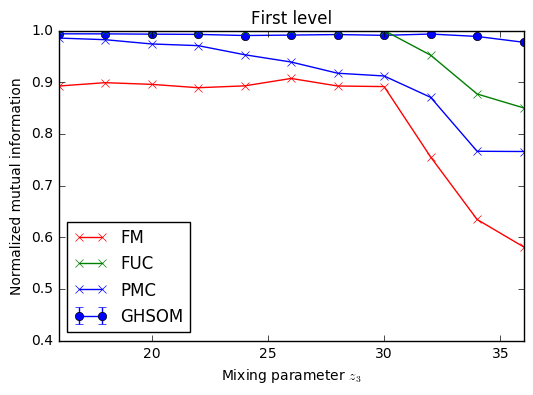
\includegraphics[scale=0.45]{first_level.png}
		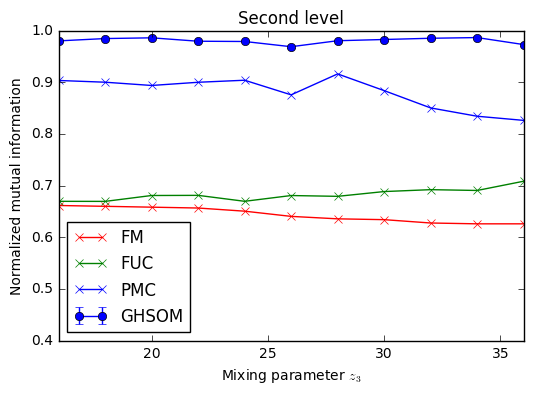
\includegraphics[scale=0.45]{second_level.png}
		\caption{Plot of mixing parameter $z_3$ against NMI score for both levels of community. 100 networks were generated with each mixing parameter. Results extracted without permission from \protect			\cite{yang2013hierarchical} (fig 4).}
\label{synthetic_experiment}
\end{figure}
\begin{itemize}
\item FM: (Fast Modularity) -- hierarchical agglomerative algorithm
(\cite{clauset2004finding})
\item FUC: (Fast Unfolding of Communities) -- heuristic method based on modularity optimization 
(\cite{blondel2008fast}).
\item PMC: (Probabilistically Mining Communities) -- models community detection as a constrained quadratic optimization problem and solves using a random walk heuristic 
(\cite{yang2013hierarchical}). 
\end{itemize}
	\end{frame}
	
	\begin{frame}[allowframebreaks]{Real world networks}
	\begin{itemize}
	\item What about real world networks?
	\item Limited to small real world benchmarks due to issues of scalability:
	\begin{itemize}
	\item Karate
	\item Dolphin
	\item Polbooks
	\item Football
	\end{itemize}
	\begin{figure}
	\centering
	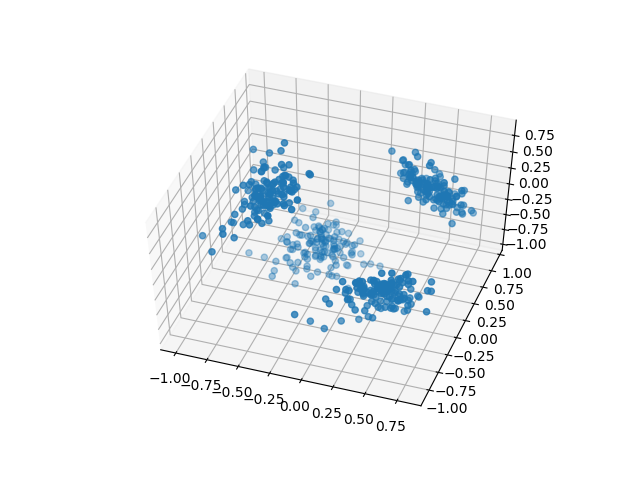
\includegraphics[scale=0.25]{3dprojection.png}
	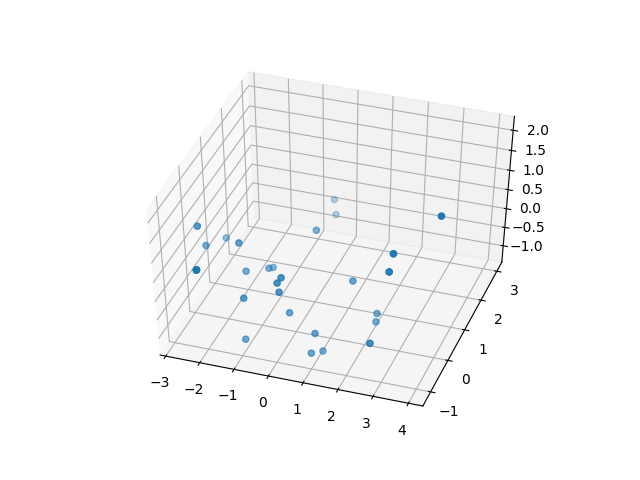
\includegraphics[scale=0.25]{3dkarate.png}
	\caption{First three dimensions of example networks embedded using MDS.}
	\end{figure}
		\item Parameter setting for the synthetic experiment was easier since the network was `regular'.
	\item Setting parameter settings for the real world networks is more challenging.
	\item A setting that was good for the karate network (with 2 labelled communities was not good for the football network (with 12 labelled communities.
	\end{itemize}
	
	\end{frame}
	
	\begin{frame}{Preliminary Results}
	\begin{table}
\centering
\begin{tabular}{ c c c c c }
\toprule
\textbf{Algorithm} & \multicolumn{4}{c}{\textbf{Network (NMI Score)}}\\
{} & Karate & Dolphin & Polbooks & Football \\ 
\bottomrule
\textbf{\#comms} & 2 & 4 & 3 & 12 \\
%\textbf{\#comms det.} & 2 & 2 & 2 & 3 \\
\bottomrule 
MCL & \textbf{1.000} & 0.424 & 0.515 & \textbf{0.935} \\ 
FM & 0.693 & 0.509 & 0.531 & 0.757 \\ 
%LP & 0.601 & 0.544 & 0.517 & 0.895 \\ 
%Infomap & 0.699 & 0.566 & 0.537 & 0.924 \\ 
FUC & 0.587 & \textbf{0.636} & \textbf{0.575} & 0.855 \\ 
%MRW & 0.562 & 0.549 & 0.543 & 0.887 \\ 
PMC & 0.837 & 0.620 & 0.574 & 0.887 \\ 
\toprule
GHSOM ($\epsilon_{sg}=0.6$) & 0.500 & 0.523 & 0.516 & 0.739 \\
GHSOM ($\epsilon_{sg}=0.8$) & 0.733 & 0.575 & 0.547 & 0.528 \\
\bottomrule
\end{tabular}
\caption{Table of NMI scores of GHSOM versus several algorithms in the literature. The best NMI score for each network is written in bold. Results for comparision algorithms are taken from \protect\cite{yang2013hierarchical} (table 2) without permission. Markov Clustering algotithm (MCL) proposed by \protect\cite{van2001graph}.}
\label{real_world_experiment}
\end{table}
	
	\end{frame}
	
	\begin{frame}[allowframebreaks]{Parameter Optimization}

\begin{table}
\centering
\begin{tabular}{l l l l l}
\bottomrule
\textbf{Parameter} & \multicolumn{4}{c}{\textbf{Network}} \\
{} & Karate & Dolphin & Polbook & Football \\
\bottomrule
%\textbf{\#jobs} & 28 & 521 & 562 & 181 \\
%\bottomrule
%$\eta$ & 0.00010 & 0.879141 & 0.999305 & 0.058690 \\
%$w$ & 0.943492 & 0.0001 & 0.352897 & 0.066269 \\
%$\sigma$ & 0.816632 & 0.001 & 0.649818 & 1.000 \\
%$\epsilon_{sg}$ & 0.988303 & 0.557975 & 0.999970 &  0.450884 \\
%$\epsilon_{en}$ & 1.000000 & 0.3 & 0.392926 & 0.300000 \\
$\eta$ & 0.0001 & 0.879 & 0.999 & 0.0587 \\
$w$ & 0.943 & 0.0001 & 0.353 & 0.0663 \\
$\sigma$ & 0.817 & 0.001 & 0.650 & 1.0 \\
$\epsilon_{sg}$ & 0.988 & 0.558 & 1.0 &  0.451 \\
$\epsilon_{en}$ & 1.0 & 0.3 & 0.393 & 0.3 \\
\bottomrule
\textbf{\#comms} & 2 & 4 & 3 & 12 \\
\textbf{\#comms det.} & 2 & 4 & 2 & 11 \\
\textbf{NMI score} & \textbf{1.0} & \textbf{0.640} & \textbf{0.688} & 0.874 \\
\bottomrule
\end{tabular}
\caption{Spearmint optimized parameter settings and NMI scores for real world networks (to 3 s.f.). Spearmint provided by \protect\cite{snoek2012practical}.}
\label{bayes}
\end{table}	
	
	\begin{itemize}
	\item This looks bad.
	\item GHSOM does not seem very robust and is dependent upon parameter settings. 
	\item But some good results, so there is potential.
	\end{itemize}
	
	\end{frame}
	
	\begin{frame}[allowframebreaks]{Towards a more principled setting of parameters}
	\begin{itemize}	
	\item Parameters:
	\begin{itemize}	
		\item $\eta$: learning rate
		\item $w$: initial weight range
		\item $\sigma$: neighbourhood function
		\item $\epsilon_{sg}$: stop map growth parameter
		\item $\epsilon_{en}$: expand parameter
	\end{itemize}
	\item Fix every parameter except the stop growth parameter $\epsilon_{sg}$.
	\item Derive equation for parameter setting $\epsilon_{sg}$ in terms of network density $\rho$.
	\end{itemize}
%	\end{frame}
%	
%	\begin{frame}
	\begin{figure}
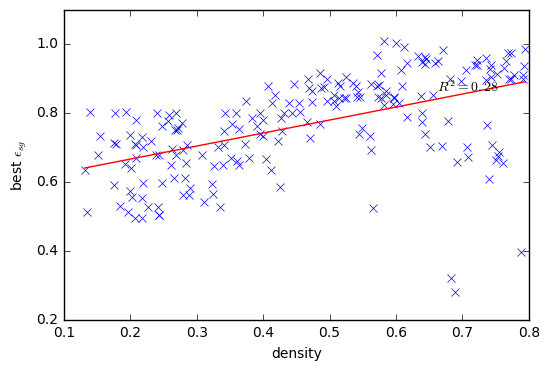
\includegraphics[scale=0.60]{derived_results.png}
\caption{Plot of network density $\rho$ vs. best setting for $\epsilon_{sg}$ found by 50 iterations of simulated annealing. 200 random networks of 64 nodes were generated with a random number of edges and communities.}
\end{figure}
%	\end{frame}
%	
%	\begin{frame}
	\begin{itemize}
	\item Derived equation: $\epsilon_{sg} = 0.377746404462 * \rho + 0.590217653032$
	\end{itemize}
	\begin{table}
	\begin{tabular}{c c c c}
	\bottomrule
	\textbf{Network} &     $\rho$  &  $\epsilon_{sg}$ &    \textbf{Mean NMI Score} \\
	\bottomrule

Karate    &  0.139037433155  &   0.642738543492  &     0.499800072199 \\

Dolphin  &   0.0840824960338   & 0.621979513587      & 0.493281211109 \\

Polbooks  &  0.0807692307692  &  0.620727939546     &  0.518261769794\\

Football  &  0.0939740655988  & 0.625716018425   &    0.733839840555\\	
	\end{tabular}
	\caption{Derived $\epsilon_{sg}$ results. Each network was repeated 100 times.}
	\end{table}
	\end{frame}
	
	\begin{frame}{A more realistic network density}
		\begin{figure}
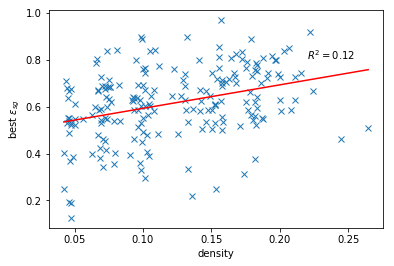
\includegraphics[scale=0.65]{derived_results_realistic.png}
\caption{Plot of network density vs. best setting for $\epsilon_{sg}$ found by 50 iterations of simulated annealing. 200 random networks of 64 nodes were generated with a random number of edges and communities. Equation: $\epsilon_{sg} = 1.002*\rho + 0.492$}
\end{figure}
	\end{frame}
	
		
	\begin{frame}{(Some of a) Discussion}
	\begin{itemize}
	\item Good when networks are regular.
	\item Very good results possible, even when mixing factor between communities is large.
	\item Parameter setting is challenging. 
	\item Looking for a more principled approach. 
	\item Poor scalability.
	\begin{itemize}
	\item Experimentation is time-consuming.
	\item Large real-world networks are infeasible.
	\item Could be efficiently parallelized. 
	\end{itemize}
	\end{itemize}
	\end{frame}
	
	\begin{frame}{What's next: Topology Preservation}
	\begin{itemize}
	\item The main advantage of SOM is topology preservation. 
	\item Similar features are mapped close together.
	\item Is this true for community detection?
	\item Will communities that are mapped together by GHSOM have similar functions?
	\item Experiment on small unlabelled biological network and compare GO terms. 
	\end{itemize}
	\end{frame}
	
	\begin{frame}[allowframebreaks]{References}
		\bibliography{references}
		\bibliographystyle{named}
	\end{frame}
	
\end{document}

